\documentclass{beamer}
\usepackage[utf8]{inputenc}

\usetheme{Madrid}
\usecolortheme{default}
\usepackage{amsmath,amssymb,amsfonts,amsthm}
\usepackage{txfonts}
\usepackage{tkz-euclide}
\usepackage{listings}
\usepackage{adjustbox}
\usepackage{array}
\usepackage{tabularx}
\usepackage{gvv}
\usepackage{lmodern}
\usepackage{circuitikz}
\usepackage{tikz}
\usepackage{graphicx}
\usepackage{multicol}

\setbeamertemplate{page number in head/foot}[totalframenumber]

\usepackage{tcolorbox}
\tcbuselibrary{minted,breakable,xparse,skins}
{
  \hbox{%
  \begin{beamercolorbox}[wd=\paperwidth,ht=2.25ex,dp=1ex,right]{author in head/foot}%
    \insertframenumber{} / \inserttotalframenumber\hspace*{2ex} 
  \end{beamercolorbox}}%
  \vskip0pt%
}
\setbeamertemplate{navigation symbols}{}

\providecommand{\nCr}[2]{\,^{#1}C_{#2}} % nCr
\providecommand{\nPr}[2]{\,^{#1}P_{#2}} % nPr
\providecommand{\mbf}{\mathbf}
\providecommand{\pr}[1]{\ensuremath{\Pr\left(#1\right)}}
\providecommand{\qfunc}[1]{\ensuremath{Q\left(#1\right)}}
\providecommand{\sbrak}[1]{\ensuremath{{}\left[#1\right]}}
\providecommand{\lsbrak}[1]{\ensuremath{{}\left[#1\right.}}
\providecommand{\rsbrak}[1]{\ensuremath{{}\left.#1\right]}}
\providecommand{\brak}[1]{\ensuremath{\left(#1\right)}}
\providecommand{\lbrak}[1]{\ensuremath{\left(#1\right.}}
\providecommand{\rbrak}[1]{\ensuremath{\left.#1\right)}}
\providecommand{\cbrak}[1]{\ensuremath{\left\{#1\right\}}}
\providecommand{\lcbrak}[1]{\ensuremath{\left\{#1\right.}}
\providecommand{\rcbrak}[1]{\ensuremath{\left.#1\right\}}}
\theoremstyle{remark}
\newtheorem{rem}{Remark}
\newcommand{\sgn}{\mathop{\mathrm{sgn}}}
\providecommand{\abs}[1]{\vert#1\vert}
\providecommand{\res}[1]{\Res\displaylimits_{#1}} 
\providecommand{\norm}[1]{\lVert#1\rVert}
\providecommand{\mtx}[1]{\mathbf{#1}}
\providecommand{\mean}[1]{E[ #1 ]}
\providecommand{\fourier}{\overset{\mathcal{F}}{ \rightleftharpoons}}
%\providecommand{\hilbert}{\overset{\mathcal{H}}{ \rightleftharpoons}}
\providecommand{\system}[1]{\overset{\mathcal{#1}}{ \longleftrightarrow}}
%\providecommand{\system}{\overset{\mathcal{H}}{ \longleftrightarrow}}
	%\newcommand{\solution}[2]{\vec{Solution:}{#1}}
%\newcommand{\solution}{\noindent \vec{Solution: }}
\providecommand{\dec}[2]{\ensuremath{\overset{#1}{\underset{#2}{\gtrless}}}}
\newcommand{\myvec}[1]{\ensuremath{\begin{pmatrix}#1\end{pmatrix}}}


\lstset{
%language=C,
frame=single, 
breaklines=true,
columns=fullflexible
}
\lstset{
  language=C,
  basicstyle=\ttfamily\footnotesize,
  keywordstyle=\color{blue}\bfseries,
  commentstyle=\color{gray}\itshape,
  stringstyle=\color{orange},
  numbers=left,
  numberstyle=\tiny\color{gray},
  breaklines=true,
  frame=single,
  showstringspaces=false,
  tabsize=4,
  captionpos=b
}
\numberwithin{equation}{section}
\lstset{
  language=Python,
  basicstyle=\ttfamily\small,
  keywordstyle=\color{blue},
  stringstyle=\color{orange},
  numbers=left,
  numberstyle=\tiny\color{gray},
  breaklines=true,
  showstringspaces=false
}

\title{Problem 2.2.23}
\author{Sarvesh Tamgade}

\date{\today} 
\begin{document}

\begin{frame}
\titlepage
\end{frame}


\section{Question}
\begin{frame}{Question}
\textbf{Question}:


\noindent Find angle \(\theta\) between the vectors \(\vec{a} = \hat{i} + \hat{j} - \hat{k}\) and \(\vec{b} = \hat{i} - \hat{j} + \hat{k}\).
   

\end{frame}

    

\section{Solution}
\begin{frame}{Solution}
\textbf{Solution:} 
\\
Express vectors in column form:
\[
\vec{a} = \myvec{1 \\ 1 \\ -1},
\qquad
\vec{b} = \myvec{1 \\ -1 \\ 1}
\]

The cosine of the angle \(\theta\) is given by:
\[
\cos\theta = \frac{\vec{a}  \vec{b}}{\|\vec{a}\| \, \|\vec{b}\|}
\]

Compute dot product:
\[
\vec{a}  \vec{b} = (1)(1) + (1)(-1) + (-1)(1) = 1 - 1 - 1 = -1
\]

Compute magnitudes:
\[
\|\vec{a}\| = \sqrt{1^2 + 1^2 + (-1)^2} = \sqrt{3}
\]
\[
\|\vec{b}\| = \sqrt{1^2 + (-1)^2 + 1^2} = \sqrt{3}
\]


\end{frame}
\begin{frame}{Solution}
    Substitute:
\[
\cos\theta = \frac{-1}{\sqrt{3}\sqrt{3}} = -\frac{1}{3}
\]
\[
\theta = \cos^{-1}\left(-\frac{1}{3}\right)
\]
\vspace{2mm}
\textbf{Answer:}

The required angle is:
\[
\boxed{\theta = \cos^{-1}\left(-\frac{1}{3}\right)}
\]
\end{frame}
\begin{frame}
    \frametitle{Graph}
    \begin{figure}[h!]
        \centering
        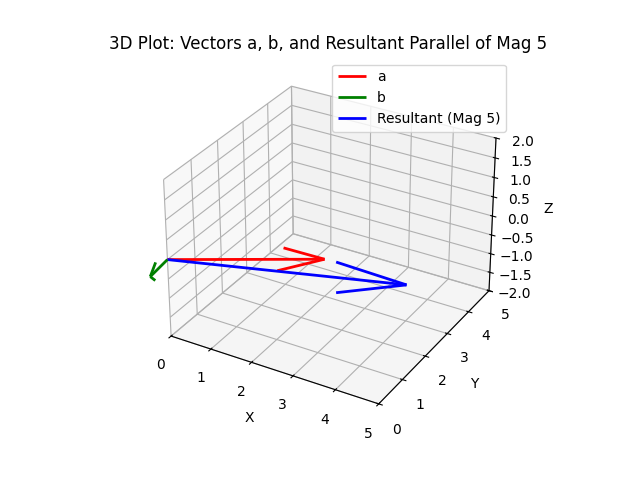
\includegraphics[width=0.7\linewidth]{FIG/graph.png}
        \caption{3D Visualisation of two vectors and angle between them}
    \end{figure}
\end{frame}
\section{ C Code}
\begin{frame}[fragile]
\frametitle{C Code }
\begin{lstlisting}[language=C]
#include <stdio.h>
#include <math.h>
#include "VectorLib.h"

int main() {
    Vector3D a = createVector(1, 1, -1);    // vector a = i + j - k
    Vector3D b = createVector(1, -1, 1);    // vector b = i - j + k

    double theta = angleBetween(a, b);  // radians

    printf("Angle between vectors a and b is %.6f radians\n", theta);
    printf("Angle between vectors a and b is %.6f degrees\n", theta * (180.0 / M_PI));

    return 0;
}

    
\end{lstlisting}
\end{frame}

\begin{frame}[fragile]
\frametitle{Python Code for Plotting}
\begin{lstlisting}[language=Python]
import numpy as np
import matplotlib.pyplot as plt

from mpl_toolkits.mplot3d import Axes3D

a = np.array([1, 1, -1])
b = np.array([1, -1, 1])
origin = np.array([0, 0, 0])

fig = plt.figure()
ax = fig.add_subplot(111, projection='3d')

ax.quiver(*origin, *a, color='r', label='a = i + j - k')
ax.quiver(*origin, *b, color='b', label='b = i - j + k')

limit = 1.5
ax.set_xlim([-limit, limit])
ax.set_ylim([-limit, limit])
ax.set_zlim([-limit, limit])

\end{lstlisting}

\end{frame}
\section{Python Code}
\begin{frame}[fragile]
\frametitle{Python Code for Plotting}
\begin{lstlisting}[language=Python]   

ax.set_xlabel('X')
ax.set_ylabel('Y')
ax.set_zlabel('Z')
ax.legend()
ax.set_title('3D Vector Plot')

plt.savefig("3d_vector_plot.png")  # Save plot to file instead of plt.show()

\end{lstlisting}

\end{frame}

\end{document}
